\chapter{Introduction and motivation}  \label{ch:introduction}
%\begin{multicols}{2}
\emph{Voxels are the future.} Volume rendering - the process of visualising voxelized data -  is a big topic and has increasingly become so over the recent years. Besides the recent rebirth of volume-based rendering in games, voxelized graphics are now ubiquitous in the special effects industry as well. The idea, however, is as old as computer graphics itself and has been pivotal in the visualisation of captured data for decades. In this first chapter we will start to outline some of the major benefits and obstacles in the world of \emph{direct volume rendering}\footnote{The authors use the term \textit{direct volume rendering} to distinguish from other forms of volume rendering where the data is converted to polygons first.}, as well as introduce the scope, scale and goals of this particular research.
%
\section{Motivation} \label{ch:inducement}
%
The compression and rendering algorithm that is presented in this thesis, is part of a larger project that is being developped at the Leiden Institute for Advanced Computer Science (LIACS). The aim is to provide a complete solution for preprocessing, storing, rendering and interacting with volumetric data sets. The main focus lies on imaging sets obtained from various microscopy scanning techniques and its potential user base would be, for example, the department of Imaging and Bioinformatics. The challenge that sets this project apart from other visualisation projects, is the fact that it is targeted at a very high-resolution display array, comparable to the work by Schwarz et al.\cite{schwarz10}. 
%
\begin{figure}[H]
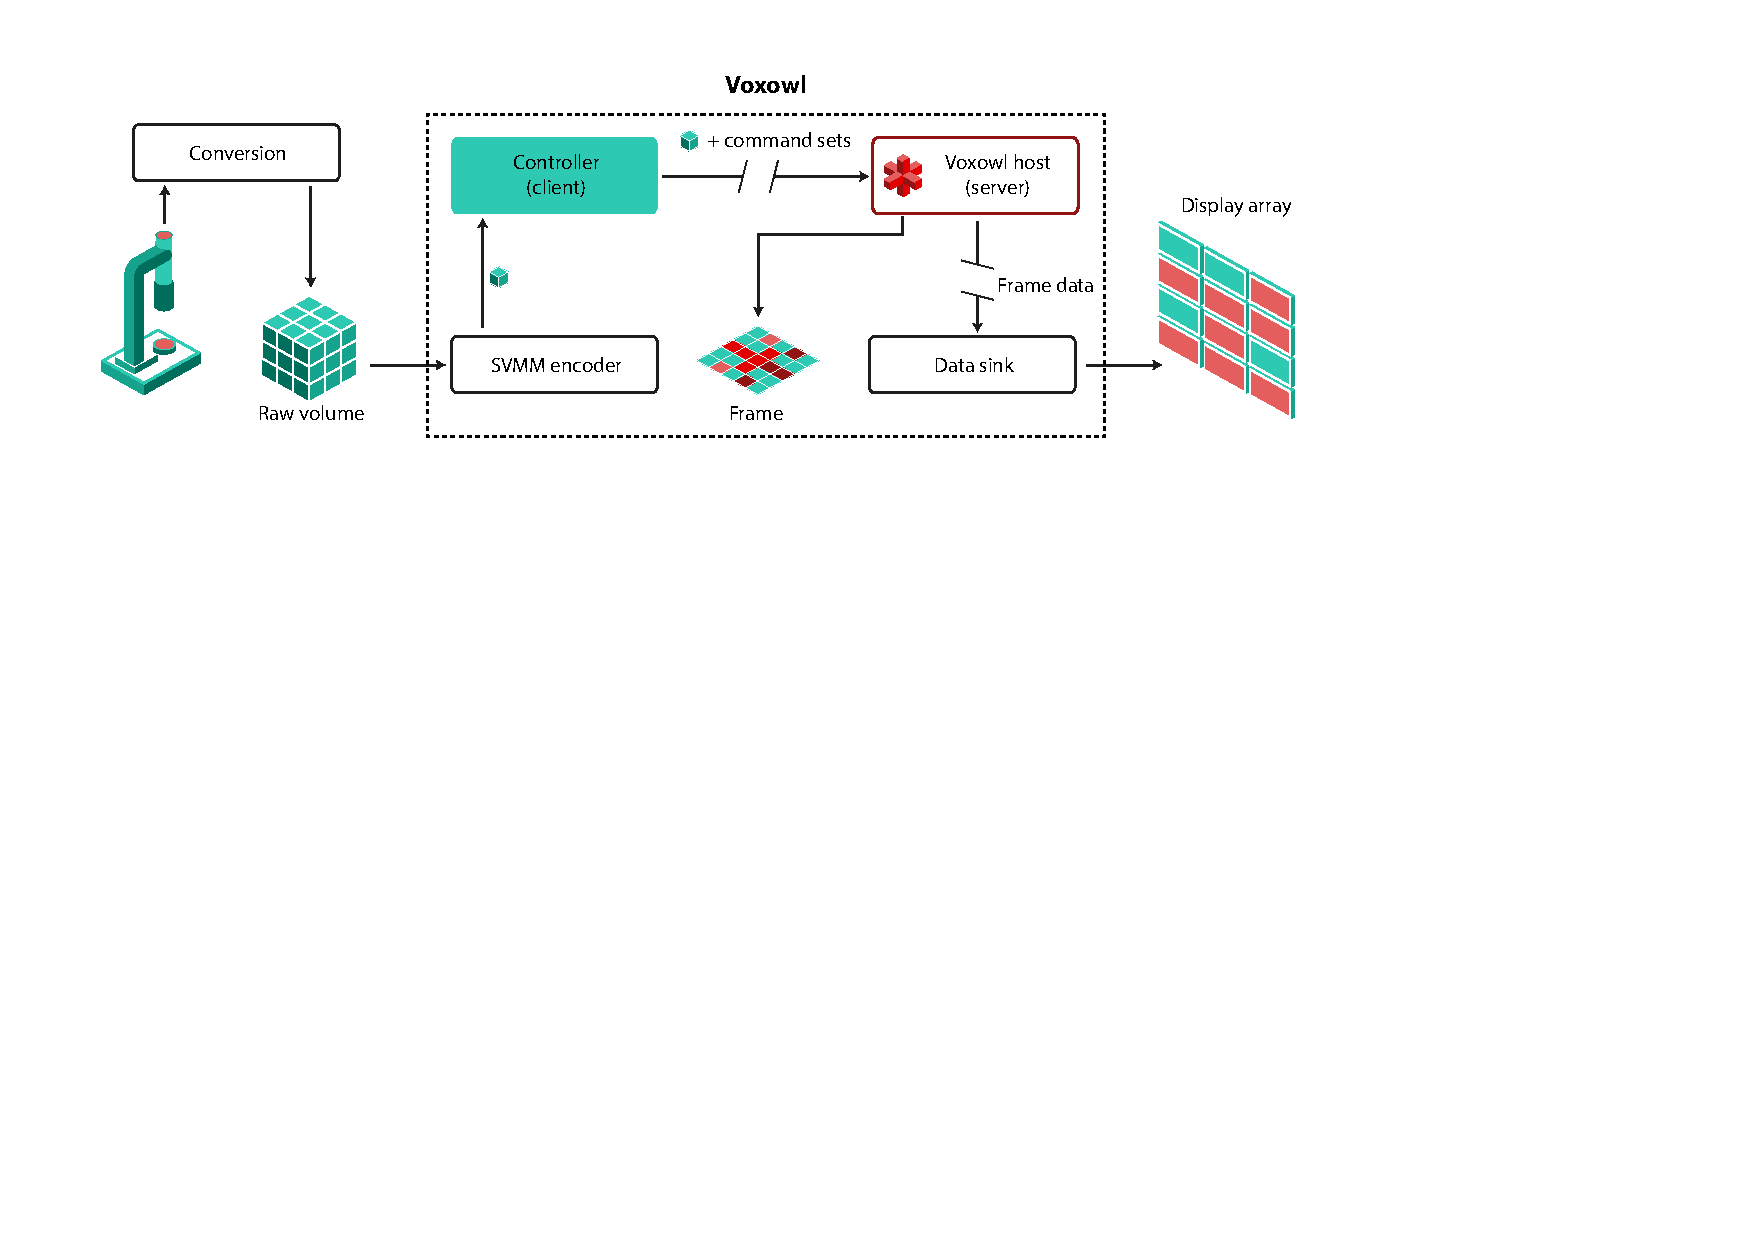
\includegraphics[scale=0.8]{figures/voxowl.pdf} 
\caption{Work flow diagram}
\label{fig:voxowl}
\end{figure}
\clearpage
%
The LIACS \emph{Big Eye} is a display array consisting of 12 large FHD displays, capable of showing a total resolution of $5760 \times 4320$ or a little over 24 megapixels. While the sheer size and detail of images are already interesting by themselves, the array presents many scientific possibilities in the exploration of data sets on a scale that could never be achieved on regular displays. For a visualisation of the envisioned work flow, see Figure \ref{fig:voxowl}.
%
\subsection{Voxowl}
\emph{Voxowl} is the name of the rendering and networking project that drives the work flow. Users are to submit their volumetric data set in compressed form from their workstation (the \emph{controller}) to the Voxowl host that runs on an external system (the \emph{server}). On this external system, multiple GPUs can be utilized to achieved interactive framerates at high resolutions while not taxing the user's workstation. Frames that are rendered, will be transmitted over a network to the display array's computer system (the \emph{data sink}). The latter can also serve as a secondary controller to request interactive manipulations (e.g. rotate or slice of the model) from the Voxowl host.

Sending images of this size over a network while minimizing the latency at the same time, can be very demanding in terms of bandwidth. An uncompressed native-resolution image for the Big Eye is a little over 71 MB if a standard \texttt{RGB8} format is utilized. When 30 frames/second are assumed for interactive exploration, a bandwidth of more than 17 Gbit/s is required. The resulting datastream must therefore be reduced in order to be transported over existing gigabit networks. Many video streaming solutions and low-latency protocols are already available for this purpose. Our reference implementation, however, uses a less sophisticated system that simply compresses each frame on an individual basis.
%
%The following sections will describe the encoding and rendering processes in more detail. More information about Voxowl, as well as a link to the source code, can be found in Appendix A.
%
\section{Direct volume rendering}
%
Informally, when one expands the idea of two-dimensional imaging into the realm of 3D, another axis is simply added to the coordinate system. Where a \textit{picture} consists of matrix of square pixels (or \textit{picture elements}), a 'volumetric picture' or \texttt{volume} consists of equally-sized, cube-shaped\footnote{A voxel does not have a particular shape defined. A cube is merely the form that maximizes the amount of space it takes in the volume.} \textit{voxels} or \textit{volume elements}. In fact, most 3D-captured (e.g., tomography, MRI) data exists in this way.

Mathematically, a volume, often called a \emph{scalar field} in that context, can be seen as a function that maps a coordinate in three-dimensional Cartesian space to a set of attributes or \emph{channels}. 
$$ f \colon \{x,y,z\} \in \mathbb{N}^{3} \to \{a_1, a_2, \dotsc, a_n\} $$
This set of attributes could be called the \emph{voxel format} (analogous to a pixel format) and usually consists of red, green, blue and alpha (color)channels. However, many more attributes are possible, such as \emph{intensity} (gray-scale channel), \emph{normals}, \emph{tangents}, \emph{bi-tangents} and contouring information. Voxel formats are often notated along with the size of the attributes, such as \texttt{RGBA32} (r, g, b and a channels of 8 bits each).

In the 80's and 90's, the first 3D computer games pioneered the use of voxels on consumer hardware\footnote{For example, Wolfenstein (1981), Commanche (1992) and Doom (1993) used a kind of raycasting based on a height-map. This is, however, not true volume rendering by today's standards.}. By that time, the CGI world had already discovered the limitations of volume-based rendering and had largely moved to polygon-based rendering. The polygon-based representation of three-dimensional objects uses arbitrarily oriented triangles in (real-valued) space. Due to their continuous nature and the fact that they can be stored by a simple set of data points, polygons hold a distinct advantage over volumes, both in the storage as well as the image quality department. Additionally, polygons can efficiently be scanline rendered, which significantly improves speed compared to the slow raycasting used on volumes. This, and the fact that around the new millennium hardware-accelerated polygon rendering became available to consumers, made volume rendering a less favorable choice. In fact, many solutions exist where the volumetric data is converted to polygons first in order to benefit from the widespread available hardware acceleration of polygon rendering.

However, direct volume rendering has a distinct set of advantages. First of all, all attributes of the image can be encoded in a uniform way. Color information, normals and texture can all be stored directly into the voxel. This enables the use of high-precision texturing without repetition. Alpha-blending is really straightforward as no depth sorting is required. For raytracing, the ray-object intersection is greatly simplified compared to polygon-based rendering. Because a voxel can either be within the field of view or not, out-of-core rendering and culling techniques are easier to implement. Lastly, scanned 3D data, such as CT or MRI scans, can be rendered without prior conversion.

Because of these advantages, the fact that storage and computing performance have improved, and that modern GPUs (see Section \ref{sec:gpgpu}) can be effectively utilized for volume rendering, volume rendering is becoming more and more commonplace. In the visual effects industry, volume rendering is not only used for effects that are inherently `volumetric', like smoke, but also lends itself well to large scenes where large amounts of low-level manipulation is required. In gaming, completely volumetric scenes are uncommon, but voxel-based techniques are often used to enhance the performance of traditional rendering (for example, voxel-based global illumination\cite{vbgi}). In the field of (scientific) visualisation - where volume rendering was already ubiquitous - images can now be manipulated interactively, see for example GigaVoxels\cite{crassin11}.

Over the years, many different direct and indirect volume rendering algorithms have been divised. For example, \emph{Splatting} \cite{qsplat} and \emph{Shear-Warp} \cite{shearwarp} are both direct methods based on mathematical transformations. An example of indirect volume rendering is the \emph{Marching Cubes} algorithm. Marching Cubes translates combinations of voxels into polygons which can be rendered using polygon-based renderers. Many more algorithms and variations exist and the reason for choosing one of them is usually a compromise between quality and speed. In this thesis, we focus completely on \emph{discrete raycasting} as it offers superior image quality.
%
\section{Discrete raycasting} \label{sec:raycasting}
%
\emph{Discrete raycasting} (or simply 'raycasting') is a volume rendering algorithm that operates by traversing the dataset along imaginary rays of light. It is among the slowest algorithms, but gives an excellent image quality. Usually, a ray is cast from every pixel on the screen and is subsequently tested for intersection with the bounding box of the volume. If such intersection occurs, the ray enters the volume from the calculated entrance point. Up until here, it is very similar to \emph{raytracing}. Raytracing operates, however, only on continuous space where as raycasting does not.

When the ray enters the volume, the volume must be traversed along the ray until either a non-transparent voxel is encountered or the volume is left on the opposite side. Traditionally, a \emph{digital differential analysis} algorithm is used to determine the next voxel that is visited by the ray. Bresenham's line algorithm \cite{bresenham65} is perhaps one of the best known algorithms for 2D grids. For volume traversal, the `3DDDA' algorithm by Fujimoto et al. \cite{fujimoto85} serves as basis for many modern algorithms, including the one by Amanatides and Woo \cite{amanatideswoo87}. Figure \ref{fig:dda} visualizes how the DDA algorithm traversel a grid.

\begin{figure*}
\centering
\begin{subfigure}{.33\textwidth}
  \centering
  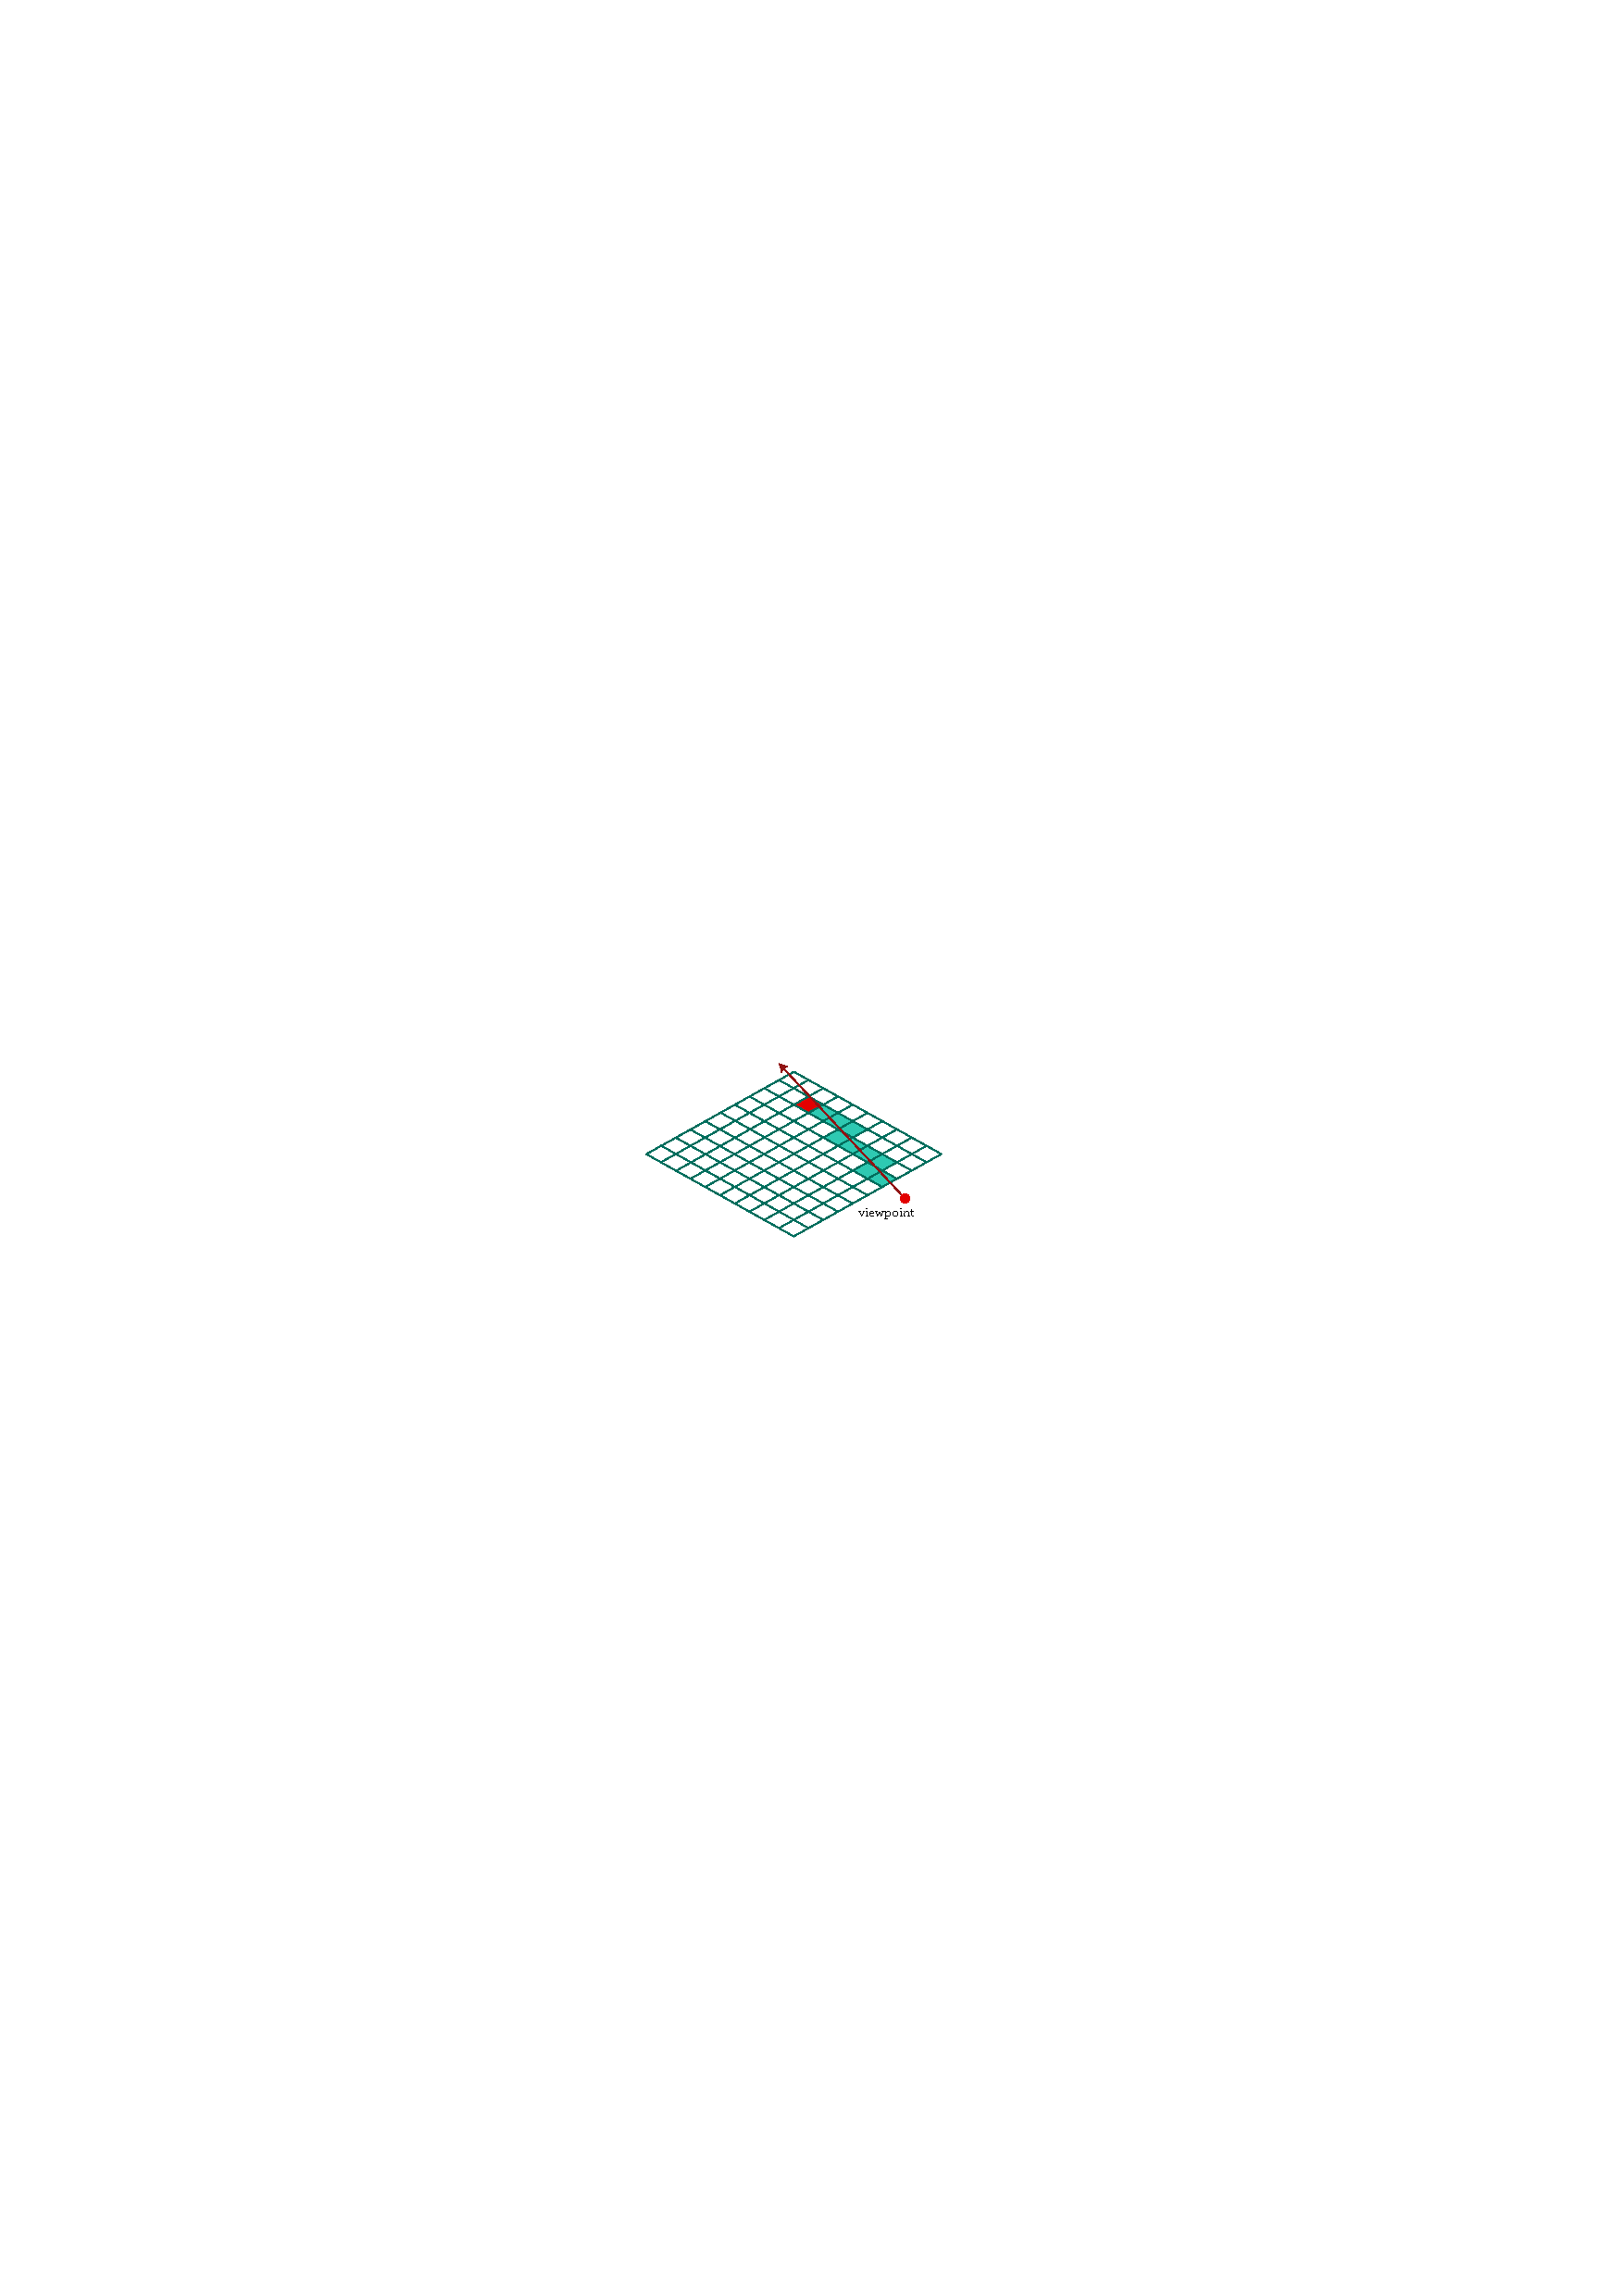
\includegraphics[scale=1]{figures/dda.pdf}
  \caption{Ray traversing a 2D grid}
  \label{fig:dda}
\end{subfigure}%
\begin{subfigure}{.33\textwidth}
  \centering
  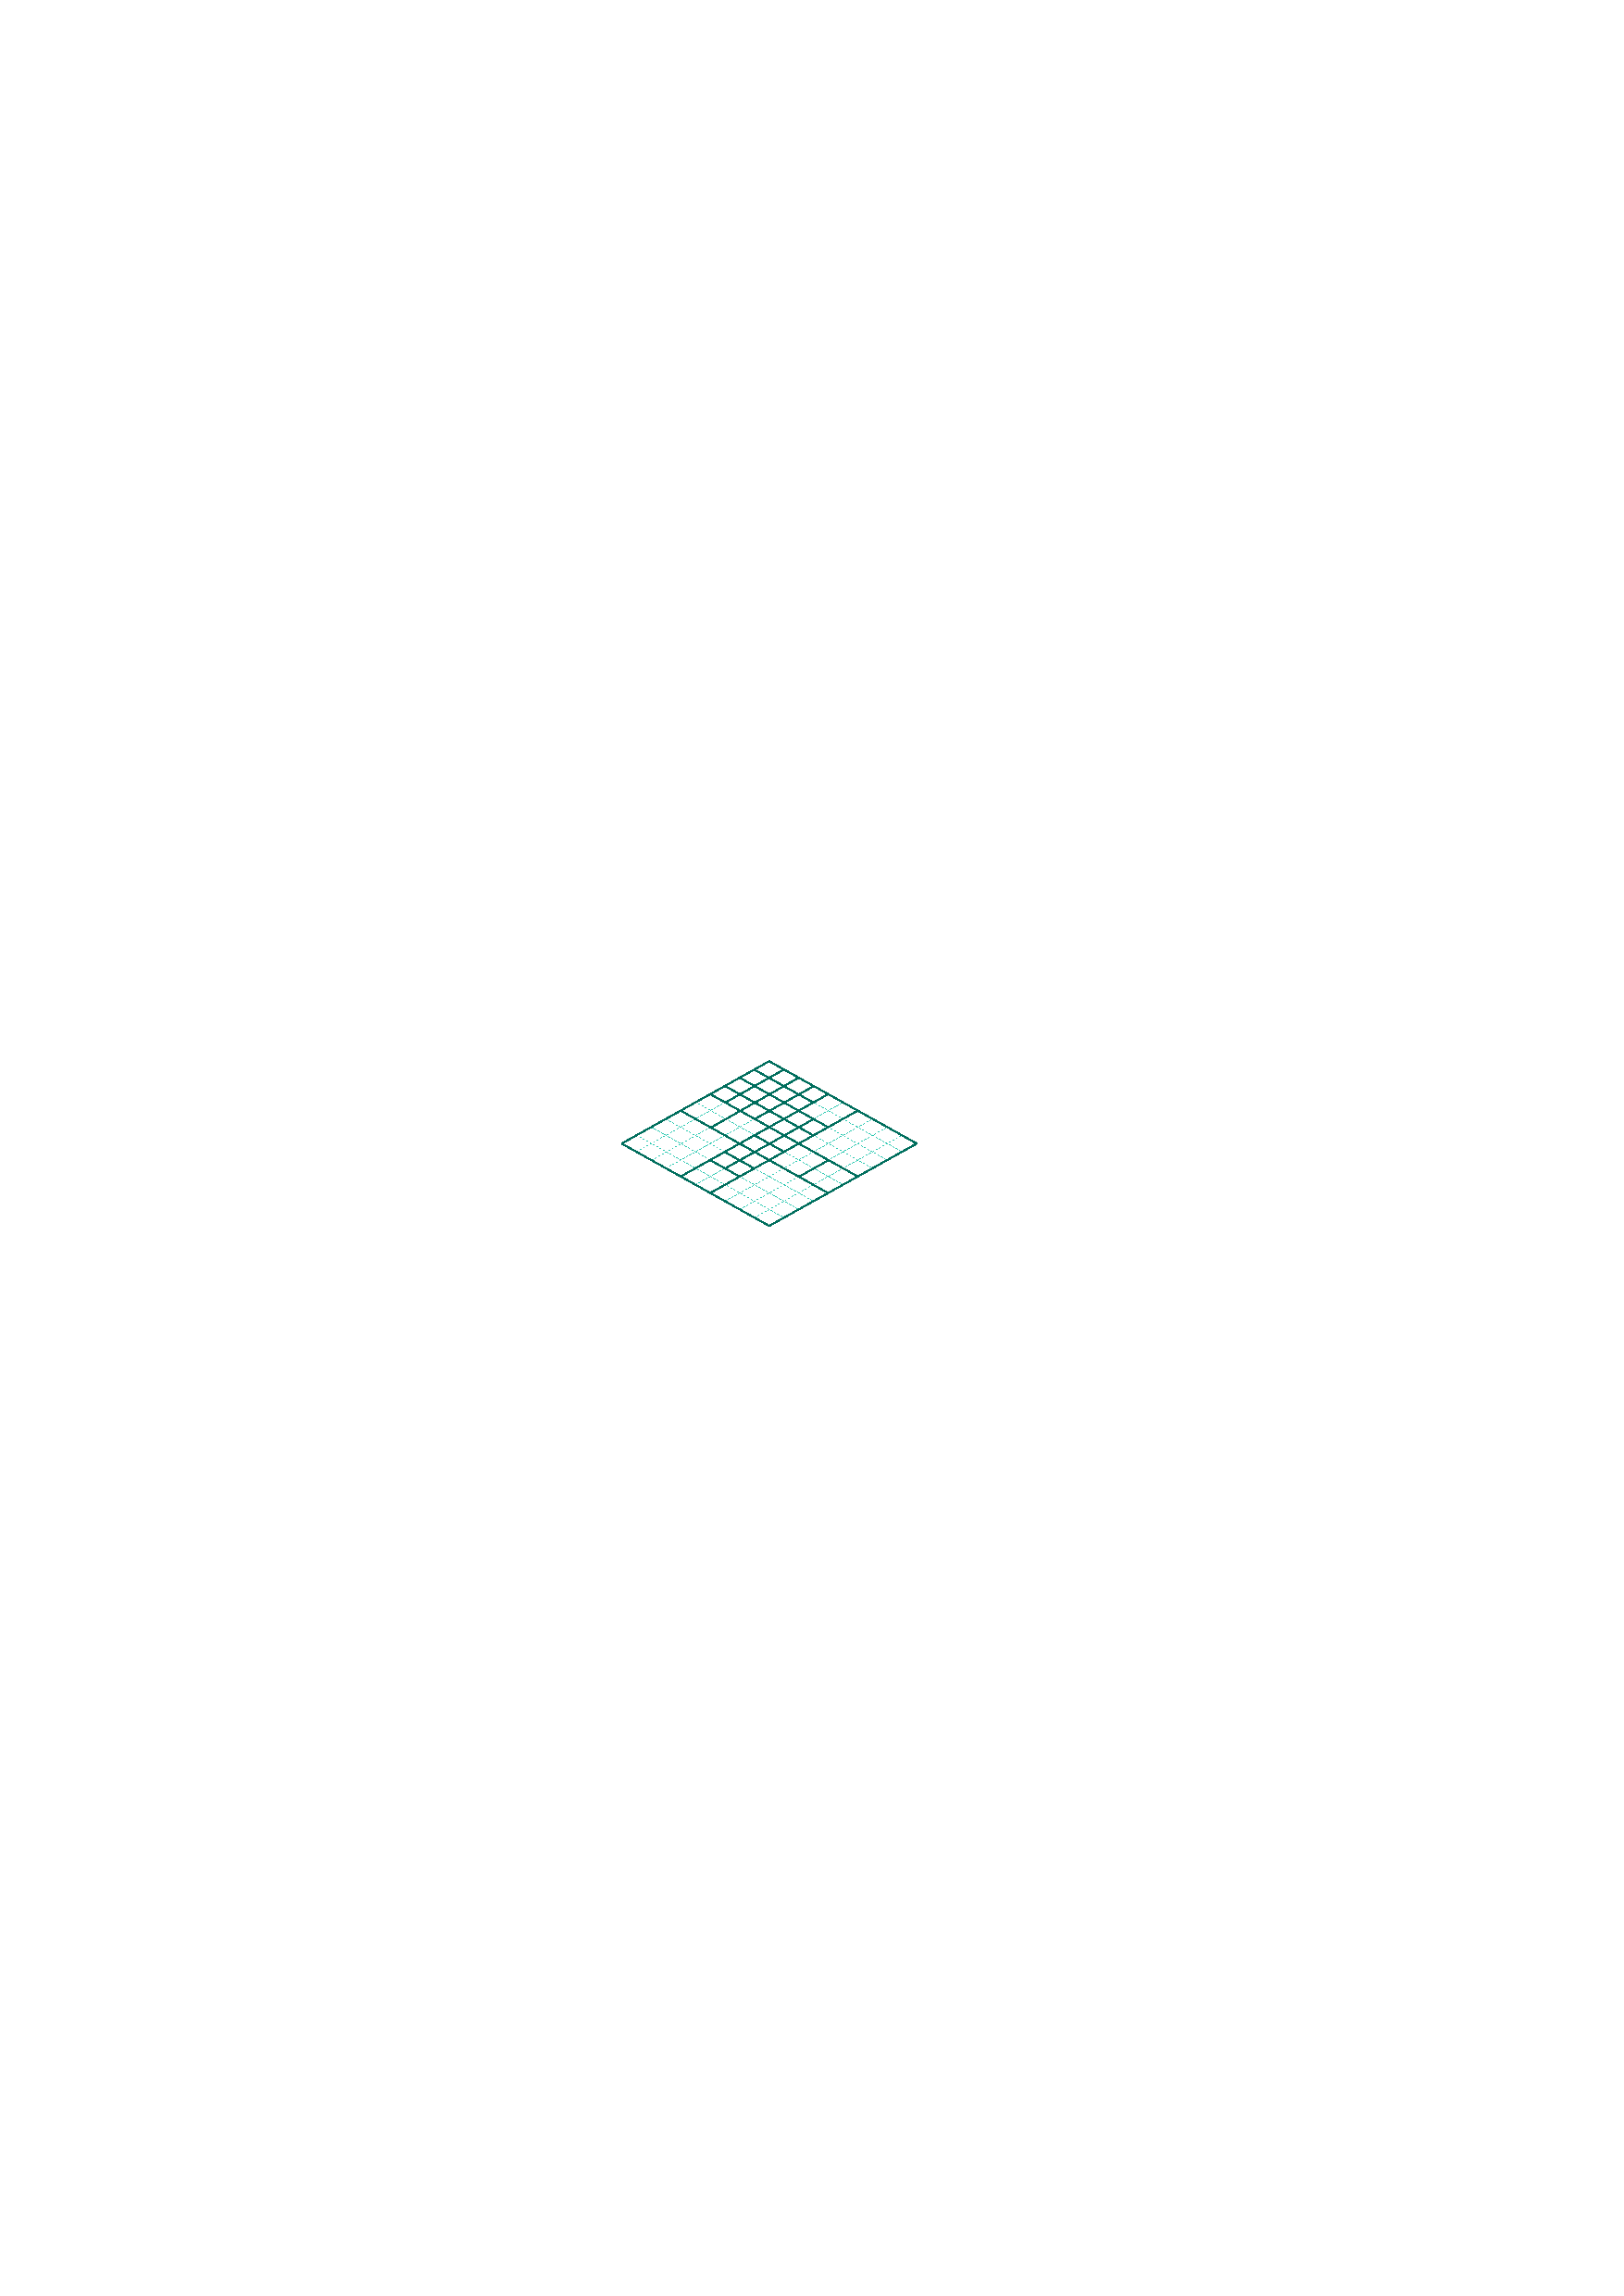
\includegraphics[scale=1]{figures/svo.pdf}
  \caption{Irregular grid of an SVO}
  \label{fig:svo}
\end{subfigure}
\begin{subfigure}{.33\textwidth}
  \centering
  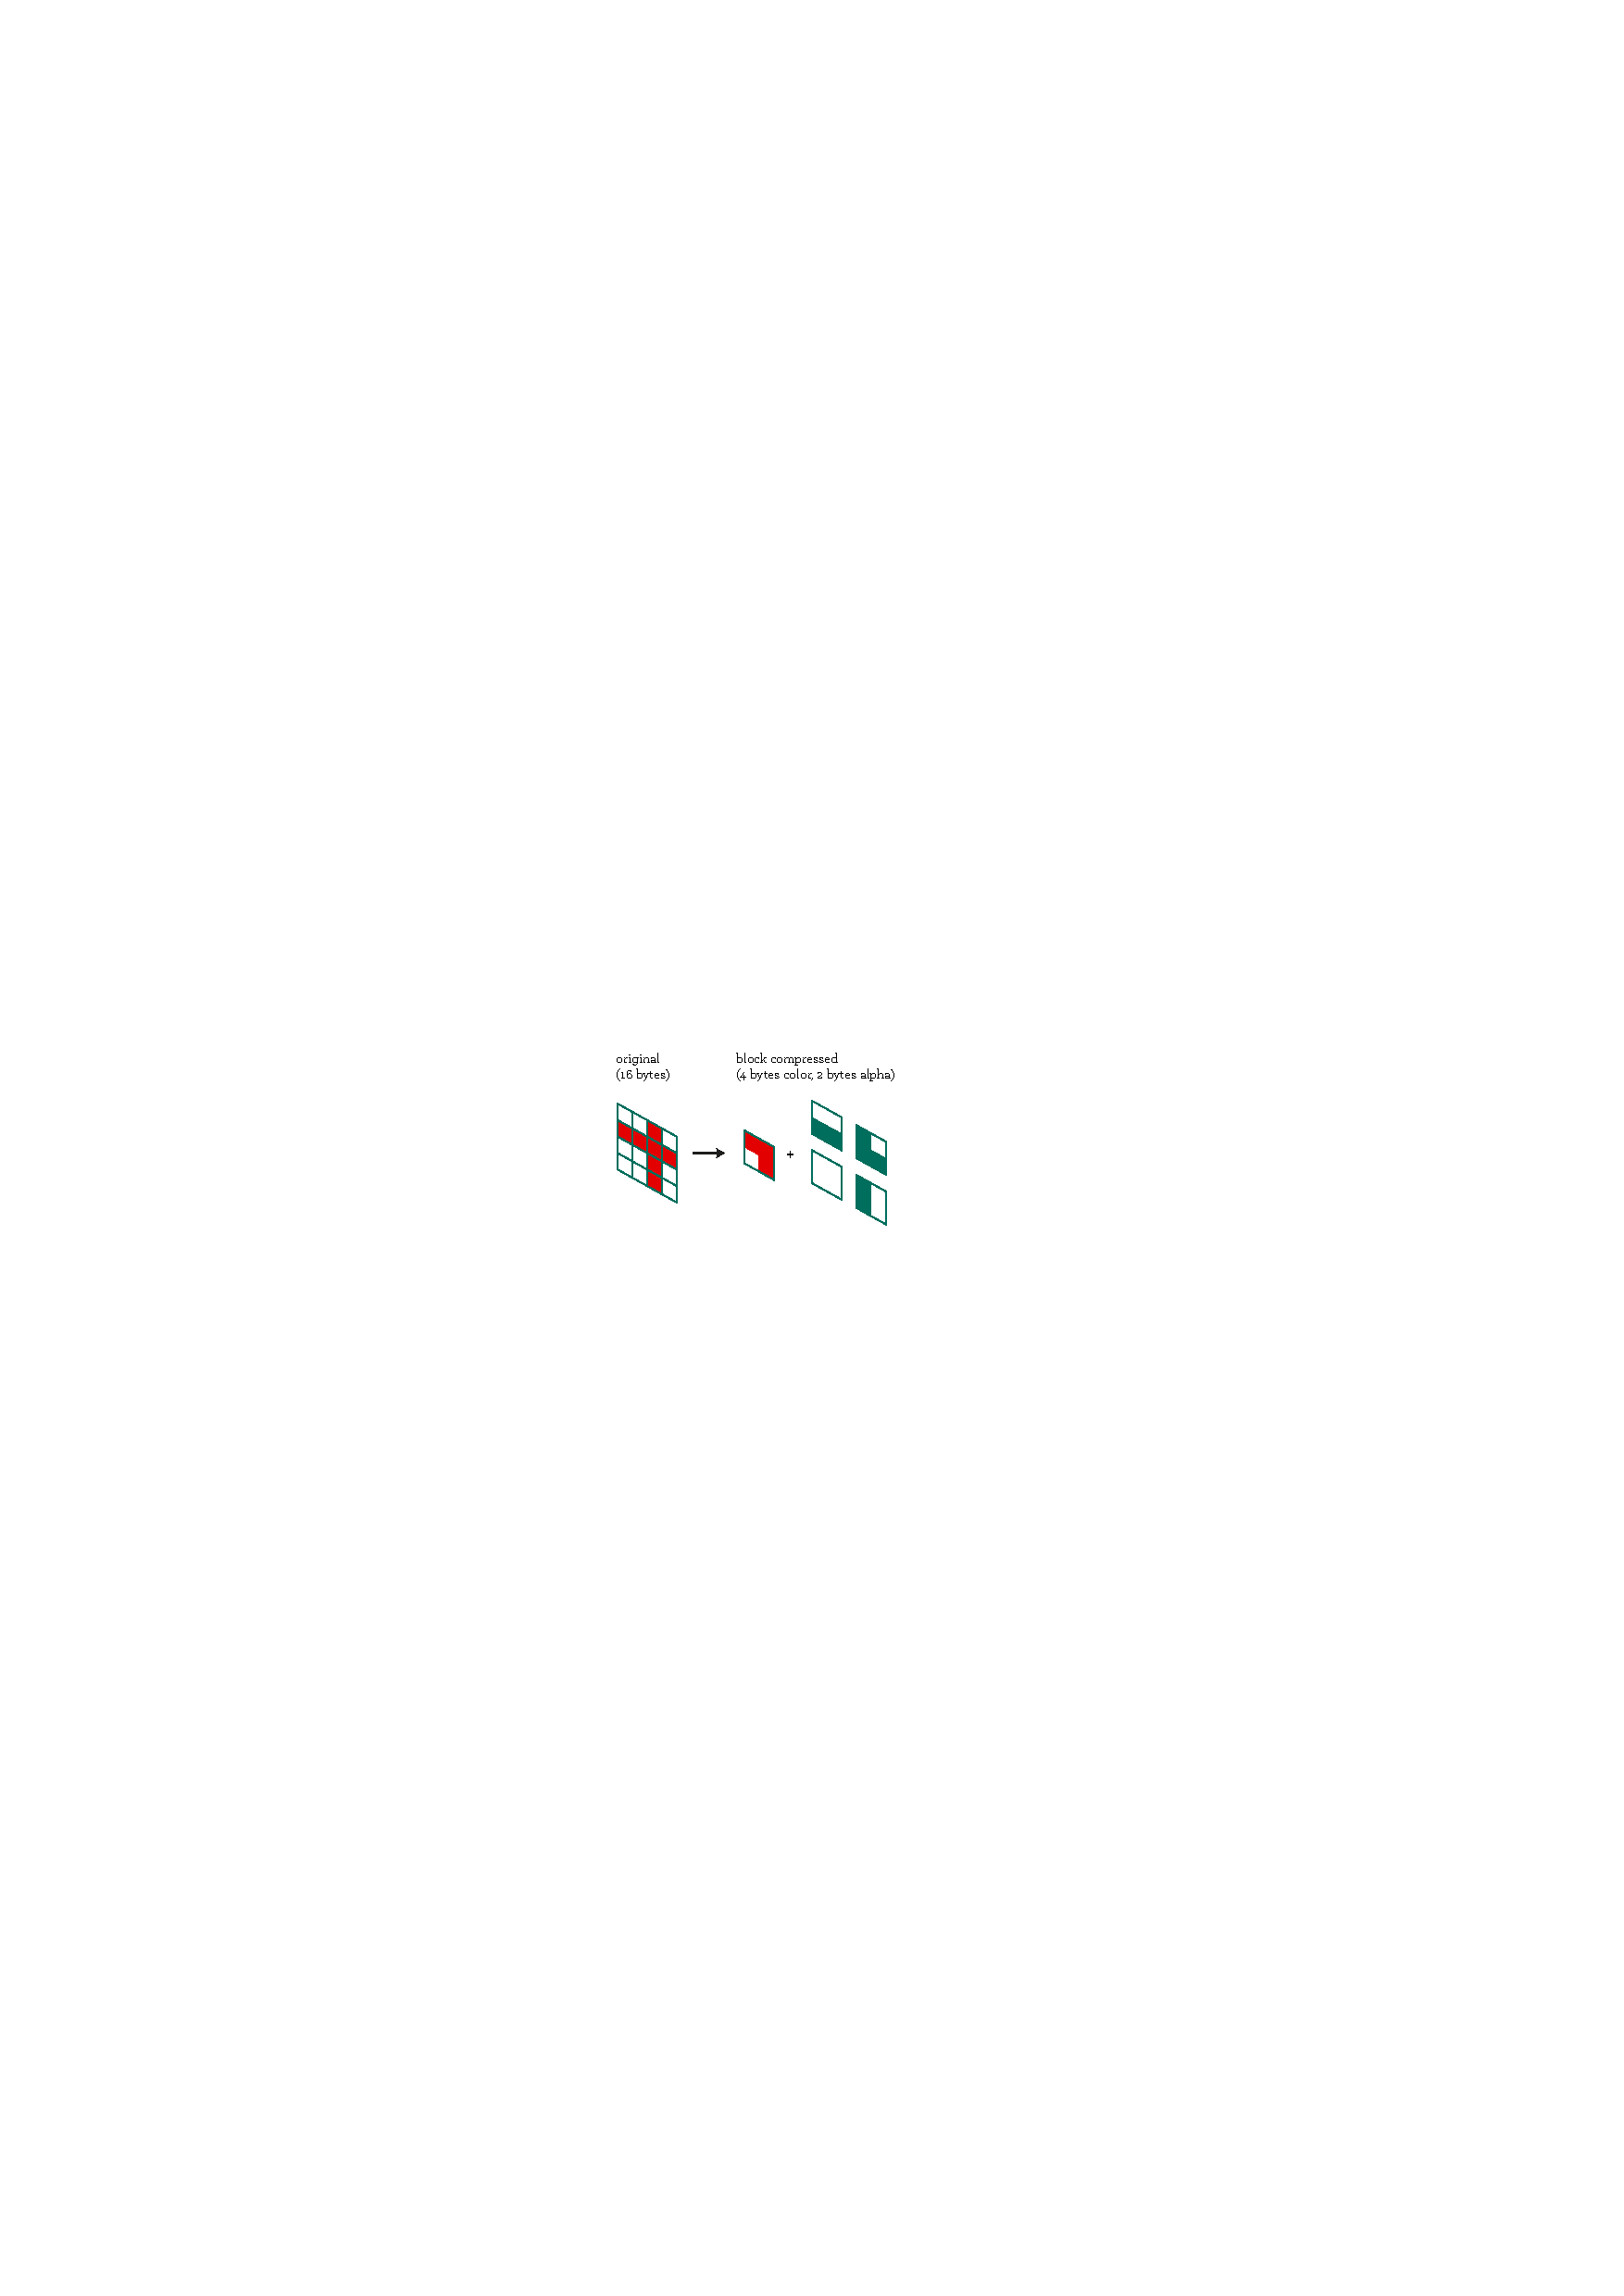
\includegraphics[scale=1]{figures/block_simple.pdf}
  \caption{Simple block compression scheme}
  \label{fig:block_bitmap}
\end{subfigure}
\caption{}
\label{fig:intro}
\end{figure*}

As we will see later in Section \ref{sec:gpgpu}, these algorithms are not directly usable in modern GPGPU computing due to heavy branching and their use of scalar operations. Many efforts exist to divise implementations that allow for efficient parallelization. In this thesis, another variation of \cite{amanatideswoo87} will be proposed that is optimized for our decompression algorithm.
%
\section{GPGPU and Cuda} \label{sec:gpgpu}
%
With the advent of \textit{general purpose GPU computing} (GPGPU for short), the graphics hardware can be programmed to almost any task, including that of direct volume rendering. \emph{Shader programs} allow specific parts of the image pipeline to be reprogrammed while leaving the rest intact. Frameworks such as OpenCL, Cg and CUDA can reprogram the \emph{stream processors} of the GPU, allow for a much greater control and are truly 'general purpose'. Both methods, and their combinations, have been successfully used to implement direct volume renderers and discrete raycasters in particular. This research mainly focusses on CUDA to implement and test the proposed algorithms on the GPU. CUDA is NVidia's proprietary GPGPU language that is developed for recent NVidia chipsets (we will use CUDA 7.5 on Maxwell generation GPUs). We will, however, attempt to generalize as much as possible, as similar results could also be achieved with other GPGPU languages such as OpenCL \cite{6047190}.

Raycasting lends itself well to implementation on the GPU. Most operations are inherently parallel, do not depend on each other and scale well. There are many obstacles, though. Algorithms that have traditionally been optimized for CPU, use as few floating-point operations (FLOPS) as possible (or replace them with integers), use many scalar operations, and rely on the CPU to efficiently handle branching. Modern GPUs however, are optimized for floating-point vector operations and perform poorly on branched code. This demands a radically different approach on code optimization. Another caveat is memory usage. While modern GPUs have several gigabytes of RAM, their memories are still a magnitude smaller than the CPU RAM. Moreover, because of its architecture and small caches, the GPU generally responds poorly to randomized access patterns to global memory.
%
\section{Voxelmap compression schemes}
%
While GPUs are in particular limited by their memory capacity, volume data tends to be large in general. For example a (not exceptionally large) voxelmap of $1024^{3}$ voxels stored in 32-bit integers requires 4 Gb of memory in an uncompressed form. This size increases cubicly with the increase of resolution and it is not uncommon for a volumetric dataset to weigh several gigabytes up to many terabytes. The naive approach would be to store this data inside a large array. Such an array will be called a \emph{voxelmap} throughout this thesis. While this method benefits from favorable constant-time access inherent to arrays, it severely limits the usable size of a dataset.  However, many effective methods of compression and encoding schemes have been developed and some of the most noteworthy will be reviewed in the following subsections.
%
\subsection{3D textures}
%
While not strictly a compression scheme, the use of the GPU's texture units give a substantial improvement in performance for direct volume rendering. Recent versions of CUDA, for example, support 3D textures with resolutions up to $2048^{3}$ and up to 128 bits of data per \emph{texel}\footnote{Analogous to a pixel in an image, the term \emph{texel} refers to one element of a texture}. Caching of these 3D textures is optimized for spatial access patterns, as opposed to regular \emph{linear memory}. This alleviates some of the problems concerning locality of ray traversal. Consider the following formula to translate a coordinate on a voxelmap $(u \in \{0,\dotsc,U-1\},v \in \{0,\dotsc,V-1\},w \in \{0,\dotsc,W-1\})$ to a linear memory position $n$. (Assuming column-major ordering)
$$
    n = w U V + v  U  + u
$$
As shown in Figure \ref{fig:dda}, ray traversal (such a 3DDDA) always accesses an adjacent voxel each step. However, to obtain for example voxel $(u,v,w+1)$, a large jump in linear memory is needed to $n+UV$.  That will be well outside any regular cache for practical sizes of $U$ and $V$. Thus for every ray cast step, a complete access to global memory is required, while wasting the entire cache at the same time (a voxel is never revisited). The hardware texture units partially solve this problem by caching `blocks' instead of linear strips of data. This and the fact that they also provide automatic padding of data to optimize the efficiency of read operations, makes 3D textures widely used for volumetric data.
\subsection{Sparse Voxel Octree}
%
Probably the most widely used datastructure for volumetric data, is the \emph{Sparse Voxel Octree} (SVO) \cite{efficientsvo10}. An octree is a tree where each node is cube-shaped and consists of $2^{3}$ child-pointers. An SVO is created by continuously subdividing the original volume by two in each direction. Thus each next level in this tree, represents an eight times larger resolution, with the bottom-level containing the original resolution and the root being a single $2^{3}$ cube. This structure can easily be compressed by iteratively removing the leaves that contain eight identical voxels. Large continuous regions are then described by a larger, top-level node, while small details are contained within the lower regions of the tree - hence the classification 'sparse'. See Figure \ref{fig:svo}.

SVOs generally give a good compression ratio at the cost of more complexity. Naturally, given a volume of size $N^{3}$, the worst-case complexity for accessing a single voxel is $log_{2}(N)$ while the average-case depends heavily on the input. To alleviate some of this increased complexity, SVOs can be used to efficiently skip empty regions by modifying the raycast algorithm. Moreover, because successive accesses are likely to have a large degree of spatial locality, the traversal of the tree can be further optimized by the use of a stack to remember parent nodes. Unfortunately, GPUs respond poorly to these optimizations due to the use of complex data structures such as a stack.
%
\subsection{Run-length encoding}
%
Run-length encoding (RLE) is another frequently used algorithm. For the sake of brevity, the principle of RLE is assumed to be known. Being a one-dimensional encoding, RLE can only be used on one axis of the voxelmap. The result is a two-dimensional grid of irregularly sized 'columns' of RLE data. RLE can be used to achieve favorable compression ratios \cite{forstmann11} while, like SVOs, it substantially increases the number of 'steps' it takes to reach a single voxel. Because compression really occurs over one axis, this complexity becomes somewhat dependent on the angle of view. RLE therefore lends itself especially well for data that already has an increased density in a certain direction, such as height maps.
%
\subsection{Transformations} \label{sec:transformations}
%
Mathematical transformations can be used to express the values of a dataset into a different domain (frequency domain is used in particular in this context). While these transformations do not compress the data as such, the resulting (transformed) data may be easier to compress with, for example, run length encoding. Moreover, a lossy compression may be achieved efficiently by leaving out the high-frequency components of the (transformed) data at a minimal degradation of the image quality. Mostly the \emph{discrete cosine transformation}\cite{cosinetransform94} and the \emph{wavelet transformation}\cite{waveletbook99} have been utilized to compress image data\footnote{JPEG and JPEG-2000 are good examples of these}.
%
\subsection{MIP maps}
%
MIP maps (MIP standing for \emph{multum in parvo}) is a technique that originates from the rendering of 2D textures. It works by recursively dividing the resolution in half and storing each subsequent downscaled image alongside the original. Each separate image is called a \emph{mipmap level}. In its original context, MIP mapping is used to enhance the filtering quality of the texture, however, in volume rendering it can be used to limit the ray traversal based on level-of-detail (LOD). For example, if parts of the image are really far away from the viewer, one of the coarser mipmap levels can be used, resulting in fewer steps when traversing the volume. In a similar fashion, inherently \emph{anti-aliased} images can be generated (\emph{ray tracing with cones})\cite{amanatides84}. For volumes, each subsequent mipmap level is only $(\frac{1}{2})^3=\frac{1}{8}$ as large as the previous level. Expanding this series gives:

$$\sum_{i=1}^{\infty} \frac{1}{8^i} = \frac{1}{7}$$

This shows that a full MIP map expansion adds only about 14,3\% to the size of the voxelmap. However, MIP maps are often combined with SVOs in this context, making the increase in size due to MIP mapping negligible.
%
\subsection{Block compression}
%
In the literature only few applications of \emph{block compression} in the field of volume rendering are described. However, this technique has many potential benefits in this area. Block compression is an umbrella term for several techniques that compress data per block of a fixed size, while producing an output with a fixed rate. The biggest advantage is that no datastructure is necessary, as regularly formatted data remains regular. This property makes it very well suited to (3D) texture compression. Disadvantages are the limited compression ratios and the inherent loss of information; block compression is a 'lossy' method by definition.

A famous example of block compression is S3TC (S3 Texture Compression) \cite{s3tc}\footnote{S3TC is currently covered by a patent that expires in 2017.}. S3TC comes in the forms of DXT1 to DXT5, all providing similar mathematical schemes of encoding a 4 $\times$ 4 block into fixed-width integers with ratios from 4:1 to 6:1. \\
In video compression, color is often separated into \emph{luminance} (brightness) and \emph{chroma} (color) channels. Owing to the fact that human vision is more sensitive to change in brightness than in color, \emph{chroma-luma} compression reduces the resolution of the chroma channel without much image degradation. Video formats often denote the applied chroma-luma compression as a ratio such as `4:2:2' or `4:2:0', giving the ratio of luminance information, horizontal-, and vertical chroma information. Figure \ref{fig:block_bitmap} shows a very simple block compression scheme inspired by `4:2:2' chroma-luma compression. The luma part is replace by a single-bit alpha channel and color is simply stored as a RGBA quadruple. We will use this scheme later in our experiments.
%
\section{Problems and questions}
%
There are many lossy compression algorithms for 2D images - both static and motion - but very few exist for volumetric data. Most existing algorithms compress their data loss-less and for the purpose of rendering only, while storage on disk and exchange over network could also greatly benefit from this compression. We also believe that loss in quality, to a degree, can be acceptable if the gain in storage requirements is large enough. As presented earlier, direct access to an array-based volume is fast but requires a significant amount out memory, while an octree-based solution sacrifices the constant-time access for a smaller memory footprint.

Our goal is to develop an improved compression scheme that could potentially be used as a means of data exchange as well as directly and without modifications during rendering. To serve as a framework and as a means of evaluations, we pose the following questions throughout this thesis:
\begin{itemize}
\item Can we devise a \emph{lossy} compression algorithm that is useful for practical volumetric data sets?
\item Can we improve upon existing methods, namely sparse voxel octrees.
\item By which factors are rendering performance, compression ratio and image quality affected? Can we find an `optimal' balance?
\item Using compression, can real-time visualisation with a large voxelmap be achieved on a single GPU? \footnote{As far as the last question is concerned, we consider an RGBA voxelmap of $2048^3$ - a little over 36 Gb - to be `large' at the time of writing. }
\end{itemize}

In addition to these questions, we hypothesize that the use of block compression will improve the size-quality ratio. We also believe that by reducing the amount of mipmap levels - or the depth of the tree in SVO-terms - the performance will improve proportionally. We will use our test result to verify these theories.
%
\section{Sparse Voxel MIP maps }
%
In an attempt to overcome the problems mentioned earlier, a novel compression data structure is proposed, that is based on SVOs, volume MIP mapping and block compression. These \emph{Sparse Voxel MIP Maps} or SVMMs are designed to efficiently make use of GPU's 3D texture memory while also limiting the amount of mipmap levels. In order to achieve compression in combination with MIP mapping, we divide the mipmap levels into individual blocks of voxels. These blocks can have an arbitrary size and can be `left out' (hence \emph{sparse}) when their entropy falls below some threshold. While we do not consider SVMM to be a tree per se, a meta-structure is intervowen into the MIP map data that much resembles an $N^3$-tree. It is using this structure that we can localize blocks in a sparsely populated mipmap level.

Some of the key-features of SVMM are: support for multiple voxel formats, efficient storage to disk and a variable lossy compression. It could potentially be expanded with out-of-core rendering (see Section \ref{sec:spatialregions}). Moreover, we make use of block compression to further reduce size and improve the size-quality ratio.
%
\section{Related Work}  \label{ch:relatedwork}
%
%\begin{multicols}{2}
%
Much research has been done into the efficient storage and level-of-detail representation of volumetric data. The use of RLE can be found in the work of Forstmann et al.\cite{forstmann11} and also in conjunction with wavelet-compression by Kim et al.\cite{wavelet99}. We will limit ourselves to SVO- and/or MIP Map based algorithms as these most directly relate to this research. For a an overview of contemporary volume compression schemes, we direct the reader to the work by Rodríguez et al.\cite{stateoftheart14}.

The work of Laine et al.\cite{efficientsvo10} describes the efficient use of SVOs for GPU rendering. Their research can be considered state of the art regarding Sparse Voxel Octrees. While their approach is very general, the decision is made to focus mainly on the surface information of the data sets. Moreover, their representation greatly benefits from \emph{contouring information} which is only available if the original data is a mesh instead of a volume. 

GigaVoxels by Crassin \cite{crassin11} appears to be a very mature project offering an all-round GPU based solution. Their efforts also include a MIP Map - SVO hybrid approach that uses a \emph{kd-start} algorithm to traverse the octree without stack and an efficient 3D texture look-up to fetch the individual voxel data. This data representation allows for \emph{ray tracing with cones}\cite{amanatides84} which provides clever anti-aliasing. Furthermore, out-of-core rendering (streaming) is utilized to allow very large data sets to be rendered on a GPU with limited memory capacity.

The work by Gobbetti et al. \cite{gobbetti08} is in many ways similar to that of Crassin \cite{crassin11}. It focussing primarily on out-of-core rendering, while the work of Crassin \cite{crassin11} discusses more facets of image quality, such as shadowing and anti-aliasing. They also implement a stack-less ray traversal algorithm, but they use a special neighbour indexing structure to achieve this. 

As far as the rendering of the compressed data - in this context by means of discrete raycasting - is concerned, the method of traversal is of great importance. It has been shown that the traversal of the volmetric data is the largest factor in throughput for direct volume rendering \cite{levoy90}. Therefore, it has been the subject of many studies. The original 3DDDA algorithm by Fujimoto et al. \cite{fujimoto85} and the subsequent improvement by Amanatides et al. \cite{amanatideswoo87} are not suited for modern GPGPU implementation. Many efforts to optimize these algorithms for \emph{stream processing} have been made, for example the work by Es et al.\cite{acceleratedgrid07}.
%
\section{Contributions}
%
In this thesis, we will discuss the theory of the proposed SVMM datastructure as well as the conceptual implementation of its encoder and decoder. We will specifically focus on optimizing the raycaster and decoder for implementation using CUDA. Since the use of GPGPU programming is now so commonplace in volumetric rendering, we believe it to be a realistic testing environment. We will also introduce the reader to our methods of evaluation and present its results. In the evaluation of our compression method, we will assess both rendering performance and compression ratio. 

The remainder of this thesis is structured as follows:
\begin{itemize}
\item Chapter \ref{ch:datastructure} will introduce the SVMM datastructure and describe its encoding
\item Chapter \ref{ch:decoding} will discus challenges encountered during decoding and rendering. It will also put the decoding in perspective by briefly touching upon the entire rendering pipeline and its potential problems.
\item In Chapter \ref{ch:evaluation}, the method of testing and its results will be elaborated on.
\item In Chapter \ref{ch:discussion} we will discuss and conclude our contribution.
\end{itemize}
%